\chapter{\difficult{Topos theory}}\label{chapter:topos}

    The main reference for this chapter is \cite{johnstone, caramello}. For an introduction to stacks and descent theory, see \cite{vistoli}.

\section{Elementary topoi}

    \newdef{Subobject classifier}{\index{subobject!classifier}
        Consider a finitely complete category (in fact, the existence of a terminal object suffices). A subobject classifier is a mono\footnote{The symbol for this morphism will become clear in Section \ref{section:internal_logic}.} $\texttt{true}:1\hookrightarrow\Omega$ from the terminal object such that for every mono $\phi:x\hookrightarrow y$ there exists a unique morphism $\chi:y\rightarrow\Omega$ that fits in the following pullback square:
        \begin{figure}[ht!]
            \centering
            \begin{tikzpicture}
                \node (A) at (0, 0) {$x$};
                \node (B) at (0, -2) {$y$};
                \node (1) at (2, 0) {$1$};
                \node (O) at (2, -2) {$\Omega$};
                \node at (1, -1) {pb};
                \draw[->] (A) -- node[above]{$\exists!$} (1);
                \draw[right hook->] (A) -- node[left]{$\phi$} (B);
                \draw[right hook->] (1) -- node[right]{$\texttt{true}$} (O);
                \draw[->] (B) -- node[below]{$\exists!\chi$} (O);
            \end{tikzpicture}
            \caption{Subobject classifier.}
            \label{fig:subobject_classifier}
        \end{figure}
    }
    \begin{adefinition}
        Consider a well-powered category $\mathbf{C}$. The assignment of subobjects $\mathrm{Sub}(x)$ to an object $x\in\ob{C}$ defines a contravariant functor $\mathrm{Sub}:\mathbf{C}\rightarrow\mathbf{Set}$. A subobject classifier $\Omega$ is a representation of this functor, i.e. the following isomorphism is natural in $x$:
        \begin{gather}
            \mathrm{Sub}(x)\cong\mathbf{C}(x,\Omega).
        \end{gather}
    \end{adefinition}

    \begin{example}[Indicator function]\index{indicator function}
        The category $\mathbf{Set}$ has a subobject classifier, the 2-element set $\{\texttt{true},\texttt{false}\}$. The morphism $\chi:S\rightarrow\Omega$ is the indicator function
        \begin{gather}
            \chi_S(x)=
            \begin{cases}
                \texttt{true}&x\in S\\
                \texttt{false}&x\not\in S.
            \end{cases}
        \end{gather}
    \end{example}

    \newdef{Elementary topos}{\index{topos!elementary}
        An elementary topos is a finitely complete Cartesian closed category admitting a subobject classifier. Equivalently, one can define an elementary topos as a finitely complete category in which all power objects exist.

        The power object $Px$ of $x\in\ob{\mathcal{E}}$ is related to the subobject classifier $\Omega$ by the following relation:
        \begin{gather}
            Px = \Omega^x.
        \end{gather}
    }
    \begin{remark}[Finite colimits]
        The original definition by \textit{Lawvere} also required the existence of finite colimits. However, it can be proven that finite cocompleteness follows from the other axioms.
    \end{remark}

    \begin{theorem}[Fundamental theorem of topos theory]\index{fundamental theorem!of topos theory}
        Let $\mathcal{E}$ be a topos. For every object $x\in\ob{\mathcal{E}}$ the slice category $\mathcal{E}/x$ is also a topos. The subobject classifier is given by $\pi_2:\Omega\times x\rightarrow x$.
    \end{theorem}

    \begin{property}[Balanced]
        All monos in a topos are regular. Hence, every mono arises as an equalizer and every epic equalizer is necessarily an isomorphism. It follows that every topos is balanced \ref{cat:balanced}.
    \end{property}

    \begin{property}[Epi-mono factorization]\index{image}
        Every morphism $f:x\rightarrow y$ in a topos factorizes uniquely as an epi followed by a mono:
        \begin{gather}
            x\overset{e}{\twoheadrightarrow}z\overset{m}{\hookrightarrow}y.
        \end{gather}
        The mono is called the \textbf{image} of $f$.
    \end{property}

\section{Internal logic}\label{section:internal_logic}

    In this subsection general finitely complete categories that admit a subobject classifier are considered (they do not have to be elementary topoi).

    \newdef{Truth value}{\index{truth value}
        A global element of the subobject classifier, i.e. a morphism $1\rightarrow\Omega$. The subobject classifier $\Omega$ is also sometimes called the \textbf{object of truth values}.
    }

    \begin{property}[Internal Heyting algebra]
        For all objects $x$ in an elementary topos, the poset of subobjects $\mathrm{Sub}(x)$ has the structure of a Heyting algebra \ref{set:heyting}. Hence, every topos canonically gives an external Heyting algebra, namely $\mathrm{Sub}(1)$. Furthermore, every power object is an internal Heyting algebra. This in particular includes the subobject classifier $\Omega=P1$.
    \end{property}

    ?? COMPLETE ??

\section{Geometric morphisms}

    \newdef{Base change}{\index{base change}
        Consider a category $\mathbf{C}$ with pullbacks. For every morphism $f:x\rightarrow y$ one can define a functor $f^*:\mathbf{C}/y\rightarrow\mathbf{C}/x$. This functor acts by pullback along $f$.
    }

    \newdef{Logical morphism}{\index{morphism!logical}
        Let $\mathcal{E},\mathcal{F}$ be (elementary) topoi. A morphism $f:\mathcal{E}\rightarrow\mathcal{F}$ is called a logical morphism if it preserves finite limits, exponential objects and subobject classifiers.
    }
    \begin{property}
        If a logical morphism has a left adjoint then it also has a right adjoint.
    \end{property}

    \newdef{Geometric morphism}{\index{morphism!geometric}\index{direct!image}\index{inverse!image}
        Let $\mathcal{E},\mathcal{F}$ be (elementary) topoi. A geometric morphism $f:\mathcal{E}\rightarrow\mathcal{F}$ consists of an adjunction \[\mathcal{E}\adj{f^*}{f_*}\mathcal{F}\] where the left adjoint is left exact. The right adjoint $f_*$ is called the \textbf{direct image} part of $f$ and the left adjoint is called the \textbf{inverse image} part. If $f^*$ itself has a left adjoint, then $f$ is said to be \textbf{essential}.
    }
    \newdef{Geometric embedding}{\index{embedding}
        A geometric morphism for which the direct image part is fully faithful.
    }
    \begin{property}[Characterization of geometric embeddings]\label{topos:characterization_embedding}
        Let $f:\mathcal{E}\rightarrow\mathcal{F}$ be a geometric embedding and let $W\subset\mathrm{hom}(\mathcal{F})$ be the collection of morphisms that are mapped to isomorphisms under $f^*$. $\mathcal{E}$ is both equivalent to the full subcategory of $\mathcal{F}$ on $W$-local objects and the localization $\mathcal{F}[W^{-1}]$ at $W$ (Definition \ref{model:localization}).
    \end{property}

    \begin{property}[Base change]
        The base change functors on a topos are logical and admit a left adjoint, the postcomposition functor. This implies that these functors can be refined to essential geometric morphisms.
    \end{property}

    \begin{example}[Topological spaces]\label{topos:topological_spaces}
        Every continuous function $f:X\rightarrow Y$ induces a geometric morphism
        \begin{gather}
            \mathbf{Sh}(X)\adj{f^*}{f_*}\mathbf{Sh}(Y),
        \end{gather}
        where the direct image functor $f_*$ is defined as
        \begin{gather}
            f_*F(U) := F(f^{-1}U)
        \end{gather}
        for any sheaf $F\in\mathbf{Sh}(X)$ and any open subset $U\in\mathbf{Open}(Y)$. The inverse image functor $f^*$ is defined using the equivalence between sheaves on topological spaces and \'etal\'e spaces. Consider a sheaf $E\in\mathbf{Sh}(Y)$ as an \'etal\'e space $\pi:E\rightarrow Y$. The inverse image of $E$ along a continuous function $f:X\rightarrow Y$ is the pullback of $\pi$ along $f$.
    \end{example}

    By the previous example the global elements $\ast\rightarrow X$ of a topological space induce geometric morphisms of the form $\mathbf{Sh}(\ast)\rightarrow\mathbf{Sh}(X)$. By noting that $\mathbf{Sh}(\ast)=\mathbf{Set}$, one obtains the following generalization:
    \newdef{Point}{\index{point}
        A point of a topos $\mathcal{E}$ is a geometric morphism $\mathbf{Set}\rightarrow\mathcal{E}$.
    }

    \newnot{Category of topoi}{
        \nomenclature[S_Topos]{$\mathbf{Topos}$}{the 2-category of (elementary) topoi and geometric morphisms}
        The category of elementary topoi and geometric morphisms is a 2-category. It is denoted by $\mathbf{Topos}$.

        In fact, to obtain the structure of a 2-category, one needs to define an appropriate notion of 2-morphism. Because a geometric morphism consists of an adjunction, one can consider two distinct conventions. Either one can choose the 2-morphisms in $\mathbf{Topos}$ to be the natural transformations $f^*\Rightarrow g^*$ (with associated transformations $g_*\Rightarrow f_*$) or one can choose them to be the natural transformations $f_*\Rightarrow g_*$ (and associated transformations $g^*\Rightarrow f^*$). This chapter follows \cite{johnstone} and the ``inverse image convention'' is used, i.e. a 2-morphism $f\Rightarrow g$ consists of natural transformations $f^*\Rightarrow g^*$ and $g_*\Rightarrow f_*$.
    }

\section{Grothendieck topos}\label{section:grothendieck_topos}

    \newdef{Sieve}{\index{sieve}
        Let $\mathbf{C}$ be a small category. A sieve $S$ on $\mathbf{C}$ is a fully faithfull discrete fibration $S\hookrightarrow\mathbf{C}$.

        A sieve $S$ on an object $x\in\mathbf{C}$ is a sieve in the slice category $\mathbf{C}/x$. This means that $S$ is a subset of $\mathrm{ob}(\mathbf{C}/x)$ that is closed under precomposition, i.e. if $y\rightarrow x\in S$ and $z\rightarrow y\in\mathrm{hom}(\mathbf{C})$, $z\rightarrow y\rightarrow x\in S$.

        All of this can be summarized by saying that a sieve on an object $x\in\ob{C}$ is a subfunctor of the hom-functor $\mathbf{C}(-,x)$.
    }

    \begin{example}[Maximal sieve]
        Let $\mathbf{C}$ be a category. The maximal sieve on $x\in\ob{C}$ is the collection of all morphisms $\{f\in\mathrm{hom}(\mathbf{C})\mid\cod(f)=x\}$ or, equivalently, all of $\mathrm{ob}(\mathbf{C}/x)$.
    \end{example}
    \begin{example}[Pullback sieve]
        Consider a morphism $f:x\rightarrow y$. Given a sieve $S$ on $y$, one can construct the pullback sieve $f^*S$ on $x$ as the sieve of morphisms in $S$ that factor through $f$:
        \begin{gather}
            f^*S(x) = \big\{g\,\big\vert\,f\circ g\in S(y)\big\}.
        \end{gather}
    \end{example}

    \newprop{Presheaf topos}{\index{presheaf!topos}\label{topos:presheaf_topos}
        Consider the presheaf category $\mathbf{Psh}(\mathbf{C})$ for an arbitrary (small) category $\mathbf{C}$. This category is an elementary topos where the subobject classifier is defined on each object in the following way:
        \begin{gather}
            \underline{\Omega}(x) := \{S\mid S\text{ is a sieve on }x\}.
        \end{gather}
        The action on a morphism $f:x\rightarrow y$ gives the morphism $\underline{\Omega}(f)$ that sends a sieve $S$ to its pullback sieve $f^*S$.

        The morphism $\texttt{true}:\underline{1}\hookrightarrow\underline{\Omega}$ is defined as the natural transformation assigning to every object its maximal sieve. For every subobject $\underline{K}\hookrightarrow\underline{X}$ the characteristic morphism $\chi_K$ is defined as follows. Consider an object $c\in\ob{C}$ and element $x\in\underline{X}(c)$. The component $\chi_K|_c$ is then given by
        \begin{gather}
            \chi_K|_c(x) := \{f\in\mathbf{C}(d,c)\mid\underline{X}(f)(x)\in\underline{K}(d)\}.
        \end{gather}
    }

    The following definition is due to \textit{Giraud} (for the original definition using the notion of a \textit{cover}, see the end of this section):
    \newdef{Grothendieck topology}{\index{Grothendieck!topology}\index{covering!sieve}
        A Grothendieck topology on a category is a map $J$ assigning to every object a collection of sieves satisfying the following conditions:
        \begin{enumerate}
            \item\textbf{Identity}\footnote{The name itself stems from the fact that the maximal sieve is generated from the identity morphism.}: For every object $x$ the maximal sieve $M_x$ is an element of $J(x)$ or, equivalently, all sieves generated by isomorphisms are in $J(x)$.
            \item\textbf{Base change}: If $S\in J(x)$, then $f^*S\in J(y)$ for every morphism $f:y\rightarrow x$.
            \item\textbf{Locality}: Consider a sieve $S$ on $x$. If there exists a sieve $R\in J(x)$ such that for every morphism $(f:y\rightarrow x)\in R$ the pullback sieve $f^*S\in J(y)$, then $S\in J(x)$.
        \end{enumerate}
        The sieves in $J$ are called ($J$-)\textbf{covering sieves}. A collection of morphisms with codomain $x\in\ob{C}$ is called a \textbf{cover}\footnote{Sometimes this term is also used to denote any collection of morphism with common codomain $x$, i.e. without reference to a covering sieve.} of $x$ if the sieve generated by these morphisms is a covering sieve on $x$.
    }
    \begin{example}[Topological spaces]
        These conditions have the following interpretation in the case of topological spaces:
        \begin{itemize}
            \item The collection of all open subsets covers a space $U$.
            \item If $\{U_i\}_{i\in I}$ covers $U$, then $\{U_i\cap V\}_{i\in I}$ covers $U\cap V$.
            \item If $\{U_i\}_{i\in I}$ covers $U$ and if for every $i\in I$ the collection $\{U_{ij}\}_{j\in J_i}$ covers $U_i$, then $\{U_{ij}\}_{i\in I,j\in J_i}$ covers $U$.
        \end{itemize}
        The canonical Grothendieck topology on $\mathbf{Open}(X)$ is given by the sieves $S=\{U_i\hookrightarrow U\}_{i\in I}$, where $\bigcup_{i\in I}U_i=U$. This topology is denoted by $J_{\mathbf{Open}(X)}$.
    \end{example}

    \newdef{Site}{\index{site}
        A (small) category equipped with a Grothendieck topology $J$.
    }

    \newdef{Matching family}{\index{matching!family}\label{topos:matching_family}
        Consider a presheaf $F\in\mathbf{Psh(C)}$ together with a sieve $S$ on $x\in\ob{C}$. A matching family for $S$ with respect to $F$ is a natural transformation $\alpha:S\Rightarrow F$ between $S$, regarded as a subfunctor of $\mathbf{C}(-,x)$, and $F$.

        More explicitly, it is an assignment of an element $x_f\in Fd$ to every morphism $(f:y\rightarrow x)\in S$ such that
        \begin{gather}
            F(g)(x_f) = x_{f\circ g}
        \end{gather}
        for all morphisms $g:z\rightarrow y$. Equivalently, a matching family for $S$ with respect to $F$ is a set of elements $\{x_f\}_{f\in S}$ such that for all covering morphisms $f:y\rightarrow x,g:z\rightarrow x\in S$ and all morphisms $f':c\rightarrow y, g':c\rightarrow z$ such that $f\circ f'=g\circ g'$ the following equations holds:
        \begin{gather}
            \label{topos:matching_family_condition}
            F(f')(x_f)=F(g')(x_g).
        \end{gather}
        Given such a matching family, one calls an element $a\in Fx$ an \textbf{amalgamation} if it satisfies
        \begin{gather}
            F(f)(a)=x_f
        \end{gather}
        for all morphisms $f\in S(y)$. The existence of such an element can also be stated in terms of natural transformations. Consider the obvious inclusion $\iota_S$ of $S$ into the the hom-functor $\mathbf{C}(-,x)$. Every morphism with codomain $x$ can be obtained from the identity morphism by precomposition and, hence, a natural transformation $\mathbf{C}(-,x)\Rightarrow F$ is determined by its action on the identity morphisms $\mathbbm{1}_x$. The existence of an amalgamation is thus equivalent to the existence of an extension of $S$ along $\iota_S$.
    }
    \remark{If the base category has all pullbacks, for example if it is a topos on its own, one can restrict the above commuting diagrams to the pullback diagrams of morphisms in the sieve $S$.}

    \newdef{Sheaf}{\index{sheaf}\index{presheaf!separated}\label{topos:sheaf}
        \nomenclature[S_Shsite]{$\mathbf{Sh}(\mathbf{C},J)$}{category of $J$-sheaves on a site $(\mathbf{C},J)$}
        Consider a site $(\mathbf{C},J)$. A presheaf $F$ on $\mathbf{C}$ is called a $J$-sheaf if every matching family for every covering sieve in $J$ admits a unique amalgamation\footnote{If there exists at most one amalgamation, the presheaf is said to be \textbf{separated}.} or, equivalently, if all sieves admit a unique extension to representable presheaves.

        The category $\mathbf{Sh}(\mathbf{C},J)$ of $J$-sheaves on the site $(\mathbf{C},J)$ is the full subcategory of $\mathbf{Psh(C)}$ on the presheaves that satisfy the above condition.
    }
    This definition can also be restated in terms of local objects \ref{cat:local_object}:
    \newadef{Sheaf}{\index{descent}\label{topos:local_object_sheaf}
        By definition every covering sieve admits a morphism into the Yoneda embedding: $\eta:S\hookrightarrow\mathcal{Y}x$. If the collection of all these morphisms is denoted by $\mathcal{S}$, a presheaf is a sheaf if and only if it is $\mathcal{S}$-local, i.e. if the following morphism is an isomorphism for all $\eta\in\mathcal{S}$:
        \begin{gather}
            Fx\cong\mathbf{Psh}(\mathcal{Y}x,F)\xrightarrow{\mathbf{Psh}(\eta, F)}\mathbf{Psh}(S,F).
        \end{gather}
        This is also called the \textbf{descent condition} for sheaves. In this context the collection of matching families $\mathrm{Match}(S,F):=\mathbf{Psh}(S,F)$ for a sieve $S$ with respect to a presheaf $F$ is often called the \textbf{descent object} of $S$ with respect to $F$.
    }

    \begin{example}[Topological spaces]
        The usual category of sheaves $\mathbf{Sh}(X)$ on a topological space $X$ is obtained as the category of sheaves on the site $(\mathbf{Open}(X),J_{\mathbf{Open}(X)})$. Since the morphisms in the covering sieves are exactly the inclusion maps $U_i\hookrightarrow U$, the pullback of two such morphisms is given by the intersection $U_i\cap U_j$. Hence, the condition for a matching family, as formulated in \ref{topos:matching_family} above, gives the second part of Definition \ref{sheaf:def}. The uniqueness of an amalgamation is equivalent to the first part of that definition.

        For topological spaces, sheaves are easily represented visually. A matching family assigns to every set $U_i$ of an open cover $\mathcal{U}\equiv\{U_i\}_{i\in I}$ of $U$ an element $x_i\in FU_i$, such that the restrictions coincide on double overlaps, as in step $(1)$ in the figure below.
        \begin{gather*}
            \begin{tikzpicture}[baseline=-1mm]
                \node (title) at (0, 2) {Cover};
                \node (Uij) at (0, 1) {$U_i\cap U_j$};
                \node (Ui) at (-1, 0) {$U_i$};
                \node (Uj) at (1, 0) {$U_j$};
                \node (U) at (0, -1) {$U$};
                \draw[left hook->] (Uij) -- (Ui);
                \draw[right hook->] (Uij) -- (Uj);
                \draw[right hook->] (Ui) -- (U);
                \draw[left hook->] (Uj) -- (U);
            \end{tikzpicture}
            \xrightarrow{\ (1)\ }
            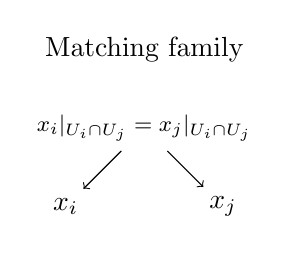
\begin{tikzpicture}[baseline=-1mm]
                \node (title) at (0, 2) {Matching family};
                \node (Uij) at (0, 1) {\footnotesize$x_i|_{U_i\cap U_j} = x_j|_{U_i\cap U_j}$};
                \node (Ui) at (-1, 0) {$x_i$};
                \node (Uj) at (1, 0) {$x_j$};
                \draw[->] (Uij) -- (Ui);
                \draw[->] (Uij) -- (Uj);
            \end{tikzpicture}
            \xrightarrow{\ (2)\ }
            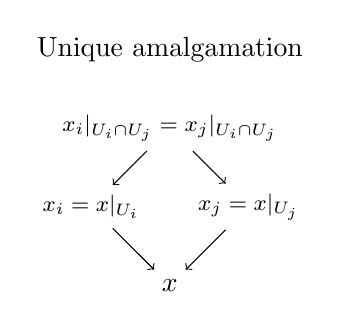
\begin{tikzpicture}[baseline=-1mm]
                \node (title) at (0, 2) {Unique amalgamation};
                \node (Uij) at (0, 1) {\footnotesize$x_i|_{U_i\cap U_j} = x_j|_{U_i\cap U_j}$};
                \node (Ui) at (-1, 0) {\footnotesize$x_i=x|_{U_i}$};
                \node (Uj) at (1, 0) {\footnotesize$x_j=x|_{U_j}$};
                \node (U) at (0, -1) {$x$};
                \draw[->] (Uij) -- (Ui);
                \draw[->] (Uij) -- (Uj);
                \draw[->] (Ui) -- (U);
                \draw[->] (Uj) -- (U);
            \end{tikzpicture}
        \end{gather*}
        The descent condition then states that for every such matching family, there exists a unique element $x$ on $U$, such that the elements of the matching family are restrictions of $x$ as in step $(2)$ of the figure above.

        The classical example would be the assignment of the set of continuous functions to open subsets of a topological space. When two functions, defined on two open sets, coincide on the intersection, there exists a unique continuous function defined on the union, such that it restricts to the given functions.
    \end{example}

    \begin{example}[Canonical topology]\index{topology!canonical}
        The canonical topology on a category is the largest Grothendieck topology for which all representable presheaves are sheaves. A subcanonical topology is then defined as a subtopology of the canonical one, i.e. any Grothendieck topology for which all representable presheaves are sheaves.
    \end{example}
    \begin{example}[Minimal and maximal topologies]
        The minimal Grothendieck topology on a category is the one for which only the maximal sieves are covering sieves. In this topology all presheaves are sheaves. The maximal Grothendieck topology is the one for which all sieves are covering sieves. In this topology only the terminal element of the associated presheaf category is a sheaf.
    \end{example}

    \newdef{Grothendieck topos}{\index{Grothendieck|seealso{topos}}\index{topos!Grothendieck}
        A category equivalent to the category of sheaves on a (small) site. This site is often called the \textbf{site of definition} for the given topos.
    }
    \begin{property}
        Every Grothendieck topos is an elementary topos.
    \end{property}

    \begin{property}
        For every Grothendieck topos there exists a site of definition for which the Grothendieck topology is (sub)canonical.
    \end{property}

    \begin{construct}[Sheafification]\index{sheafification}
        Given a presheaf $\mathcal{F}$, one can construct a sheaf $\overline{\mathcal{F}}$ along the same lines of Construction \ref{sheaf:colimit_construction}.
    \end{construct}

    \newdef{Global sections functor}{\index{global!sections}\label{topos:global_sections}
        Every Grothendieck topos $\mathcal{E}$ admits a geometric morphism to $\mathbf{Set}$, where the right adjoint assigns to an object $x$ its set of global elements:
        \begin{gather}
            \Gamma:\mathcal{E}\rightarrow\mathbf{Set}:x\mapsto\mathcal{E}(1,x).
        \end{gather}
        When $\mathcal{E}$ is the sheaf topos over a topological space, this is exactly the global sections functor \ref{sheaf:global_sections_functor}. The left adjoint assigns to every set $S$ the copower $S\cdot1\equiv\bigsqcup_{s\in S}1$. When $\mathcal{E}$ is a sheaf topos, this adjoint is exactly the constant sheaf functor. It is sometimes denoted by $\mathrm{LConst}$.
    }

    A different approach for defining sheaf topoi is through an embedding of sheaves into presheaves.
    \newdef{Local isomorphism}{\index{local!isomorphism}
        A system of local isomorphisms in $\mathbf{Psh(C)}$ is a class of morphisms in $\mathbf{Psh(C)}$ forming a system of weak equivalences \ref{model:weak_equivalence} closed under pullbacks along morphisms out of representable presheaves.
    }
    \begin{property}[Local isomorphisms and Grothendieck topologies]
        A system of local isos induces a \textit{system of local epis} in the following way. $f:X\rightarrow Y$ is a local epi if $\im(f)\rightarrow Y$ is a local iso. A Grothendieck topology is defined by declaring a presheaf $F\in\mathbf{Psh(C)}$ to be a covering sieve at $X\in\ob{C}$ if $F\hookrightarrow\mathcal{Y}X$ is a local epi.
    \end{property}

    \newadef{Sheaf topos}{\index{topos!sheaf}
        A category $\mathbf{Sh(C)}$ equipped with a geometric embedding into $\mathbf{Psh(C)}$.
        \begin{proof}[Proof of equivalence]
            By Property \ref{topos:characterization_embedding} such a category is equivalent to the full subcategory on $S$-local presheaves for some system of local isomorphisms $S$ and, therefore, also to a sheaf topos in the sense of Grothendieck by the property above.
        \end{proof}
    }
    \begin{remark}[Descent condition]
        This is essentially a restatement of the descent condition \ref{topos:local_object_sheaf}. Covering sieves, regarded as subfunctors, are in particular local isomorphisms. Stability of sieves under pullback together with the co-Yoneda lemma \ref{cat:ninja_yoneda}, which says that every presheaf is a colimit of representables, generates the full collection of local isomorphisms.
    \end{remark}

    As a last point the weaker notion of coverages is introduced:
    \newdef{Coverage}{\index{coverage}\label{topos:coverage}
        Let $\mathbf{C}$ be a category. A coverage on $\mathbf{C}$ is a map that assigns to every object $x\in\ob{C}$ a collection of families $\{f:y\rightarrow x\}\subset\mathrm{hom}(\mathbf{C})$ satisfying the following condition. If $\{f:y\rightarrow x\}$ is a \textbf{covering family} on $x$, then for every morphism $g:x'\rightarrow x$ there exists a covering family $\{f':y'\rightarrow x'\}$ on $x'$ such that every composite $g\circ f'$ factors through some $f$.
    }
    It should be clear that every coverage generates a sieve (the smallest sieve containing the coverage). Furthermore, although coverages are weaker and easier to handle, they are in fact equivalent for the purpose of sheaf theory:
    \begin{property}
        Consider a covering family $C$ and let $S_C$ be the sieve it generates. A presheaf is a sheaf for $C$ if and only if it is a sheaf for $S_C$.
    \end{property}

\subsection{Topological sheaves}

    See Chapter \ref{chapter:sheaf} for the application of sheaves to topology.

    \begin{property}[Presheaf topos]\label{topos:sheaf_topos}
        Consider the presheaf category \[\mathbf{Psh}(X):=\mathbf{Psh(Open}(X))\] over a topological space $(X,\tau)$. Unpacking Property \ref{topos:presheaf_topos} shows that this category is an elementary topos where the subobject classifier $\Omega$ is defined as follows:
        \begin{gather}
            \Omega(U) := \{V\in\tau\mid V\subseteq U\}.
        \end{gather}
    \end{property}

    \begin{construct}[Sheaves and \'etal\'e bundles]\label{topos:etale_adjunction}
        Let $X$ be a topological space. The functor \[I:\mathbf{Open}(X)\rightarrow\mathbf{Top}/X:U\mapsto(U\hookrightarrow X)\] induces the following adjunction:
        \begin{gather}
            \mathbf{Top}/X\adj{E}{\Gamma}\mathbf{Psh}(X).
        \end{gather}
        The slice category on the right-hand side is the category of (topological) bundles (Chapter \ref{chapter:bundles}) over $X$. Both directions of the adjunction have a clear interpretation. The right adjoint assigns to every bundle its sheaf of local sections and the left adjoint assigns to every presheaf its bundle of germs.

        By restricting to the subcategories on which this adjunction becomes an adjoint equivalence, one obtain the \textbf{\'etal\'e space} and \textbf{sheaf categories} respectively:
        \begin{gather}
            \mathbf{Et}(X)\cong\mathbf{Sh}(X).
        \end{gather}
        The category on the right-hand side is the category of sheaves on a topological space $X$. The category on the left is the full subcategory on local homeomorphisms, i.e. the \'etal\'e spaces \ref{topology:etale_space}.
    \end{construct}

    \begin{property}[Associated sheaf]
        The inclusion functor $\mathbf{Sh}(X)\hookrightarrow\mathbf{Psh}(X)$ admits a left adjoint, the sheafification functor that assigns to every presheaf its associated sheaf. This functor is given by the composition $\Gamma\circ E$, which is just Construction \ref{sheaf:etale_construction}.

        The fact that the counit of the adjunction \ref{topos:etale_adjunction} restricts to an isomorphism on the full subcategory $\mathbf{Sh}(X)$ is equivalent to the fact that the sheafification of a sheaf $\Gamma$ is again $\Gamma$.
    \end{property}

    \newdef{Petit and gros topoi}{\index{topos!petit \& gros}
        Consider a topological space $X$ together with its category of opens $\mathbf{Open}(X)$. The petit topos over $X$ is defined as the sheaf topos $\mathbf{Sh}(X)$. It represents $X$ as some kind of generalized space. (By Construction \ref{topos:etale_adjunction} the objects in a small topos are the \'etal\'e spaces over a given base space.) However, one can also build a topos whose objects are generalized spaces. To this end, choose a site $S$ of ``probes'' and call the sheaf topos $\mathbf{Sh}(S)$ a gros topos. See Section \ref{section:smooth_spaces} for more information.
    }

    \begin{property}[Localic reflection]\index{localic reflection}
        Mapping a topological space to its sheaf of continuous sections defines a functor $\func{\mathbf{Sh}}{Top}{Topos}$ by Example \ref{topos:topological_spaces}. When restricted to the full subcategory of sober spaces \ref{topology:sober_space}, this functor becomes fully faithful. Generalizing to sober locales even gives a reflective inclusion \ref{cat:reflective_inclusion}.

        This property states that no information is lost when regarding (sober) topological spaces as sheaf topoi. This also explains the name ``petit topos''.
    \end{property}

\subsection{Lawvere-Tierney topology}

    \newdef{Lawvere-Tierney topology}{\index{Lawvere-Tierney}
        As noted in Section \ref{section:internal_logic} on the internal logic of elementary topoi, the subobject classifier $\Omega$ has the structure of an internal Heyting algebra and, in particular, that of a meet-semilattice, where the meet is given by the pullback of morphisms. This internal poset, viewed as an internal category, admits the construction of a closure operator $j:\Omega\rightarrow\Omega$ (Definition \ref{cat:closure_operator}) satisfying the following condition:
        \begin{gather}
            j\circ\land = \land\circ(j\times j).
        \end{gather}
        This condition states (in a nontrivial way) that $j$ is (internally) order-preserving.
    }
    \begin{remark}
        The condition satisfied by the unit morphism in the definition of a closure operator can also be reformulated in this context as follows:
        \begin{gather}
            j\circ\texttt{true} = \texttt{true}.
        \end{gather}
    \end{remark}
    The Lawvere-Tierney operator also induces a ``closure operator'' on all posets $\mathrm{Sub}(x)$ in the topos. Given an object $x$ and a subobject $u\in\text{Sub}(x)$, one defines the closure $j_\ast(u)\in\text{Sub}(x)$ as the subobject classified by the characteristic morphism $j\circ\chi_u:x\rightarrow\Omega$.

    \newdef{Dense object}{\index{dense}
        Given a Lawvere-Tierney topology $j:\Omega\rightarrow\Omega$, a subobject $u\in\text{Sub}(x)$ is said to be dense (in $x$) if it satisfies $j_\ast(u)=x$.
    }
    \newadef{Sheaf}{\index{sheaf}
        Given a Lawvere-Tierney topology $j:\Omega\rightarrow\Omega$ on a topos $\mathcal{E}$, one calls an object $s\in\ob{\mathcal{E}}$ a $j$-sheaf if for all dense morphisms $u\hookrightarrow x$ the induced map \[\mathcal{E}(x,s)\rightarrow\mathcal{E}(u,s)\] is a bijection.
    }

    \begin{property}
        For the presheaf topos on a small category $\mathbf{C}$, the Grothendieck topologies on $\mathbf{C}$ and Lawvere-Tierney topologies on $\mathbf{Psh(C)}$ are equivalent.
        \begin{proof}[Sketch of proof]
            Since a Grothendieck topology assigns to every object a collection of sieves, Property \ref{topos:presheaf_topos} implies that $J(x)\subseteq\Omega_\mathbf{Psh}(x)$ for all $x\in\ob{C}$. By the base change condition of Grothendieck topologies, this relation is natural in $x$ and, hence, $J$ is a subobject of $\Omega_\mathbf{Psh}$. One thus finds a characteristic morphism $j:\Omega_\mathbf{Psh}\rightarrow\Omega_\mathbf{Psh}$ that can be proven (by the other conditions of Grothendieck topologies) to define a Lawvere-Tierney topology on $\mathbf{Psh(C)}$. Conversely, a Lawvere-Tierney topology is a morphism $j:\Omega\rightarrow\Omega$ and, hence, determines a unique subobject of $\Omega_\mathbf{Psh}$, i.e. a unique collection of sieves for every object $x\in\ob{C}$. From the conditions of Lawvere-Tierney topologies one can then prove that this collection satisfies the conditions of a Grothendieck topology.
        \end{proof}
    \end{property}
    \remark{It follows that Lawvere-Tierney topologies generalize Grothendieck topologies from presheaf topoi to arbitrary elementary topoi.}

\section{Stacks}\index{stack}
\subsection{2-sheafs}

    An important subject, especially in the context of gauge theories in physics, is that of groupoid-valued (pre)sheaves. To this end, sites are generalized to higher category theory.
    \newdef{2-presheaf}{\index{presheaf}\index{prestack}
        Consider a 2-category $\mathbf{C}$. A 2-presheaf on $\mathbf{C}$ is a pseudofunctor $\cfunc{F}{C}{Cat}$. When $\mathbf{C}$ is the categorification of a 1-category, i.e. when it has discrete hom-categories, 2-presheaves are better known as \textbf{prestacks}.
    }
    \newdef{2-coverage}{\index{coverage}\index{site}
        Virtually the same as an ordinary coverage \ref{topos:coverage}, but factorization is only required to exist up to an isomorphism. A 2-category equipped with a 2-coverage is called a \textbf{2-site}.

        As for 1-sites, every coverage generates a unique sieve. It is the full subcategory on those morphisms that factor through a covering map in the given coverage (again up to isomorphism).
    }
    As in the case of ordinary categories (Definition \ref{topos:local_object_sheaf}), one can define 2-sheaves through a descent condition:
    \newdef{2-sheaf}{\label{topos:2_sheaf}
        A 2-presheaf $\cfunc{F}{C}{Cat}$ on a 2-site $(\mathbf{C},J)$ is said to be a 2-sheaf with respect to $J$ if for all sieves $S\in J$ the following functor is an equivalence:
        \begin{gather}
            Fc\cong\mathbf{Psh}_2(\mathcal{Y}c,F)\rightarrow\mathbf{Psh}_2(S,F),
        \end{gather}
        where the fist equivalence is just the 2-Yoneda lemma.
    }
    \begin{remark}
        It should be noted that 2-(pre)sheaves can also be defined on ordinary (1-)sites. Sieves, regarded as subfunctors of the Yoneda embedding, take values in $\mathbf{Set}$. By composing these with the embedding $\mathbf{Set}\hookrightarrow\mathbf{Cat}$ of sets as (discrete) categories, one obtains 2-subfunctors of the 2-Yoneda embedding. Often 2-sheaves over 1-sites are called \textbf{stacks} (although this terminology is also used for general 2-sites).
    \end{remark}

    \newdef{Prestack of groupoids}{
        Consider a category $\mathbf{C}$. A prestack of groupoids on $\mathbf{C}$ is a $\mathbf{Grpd}$-valued prestack on $\mathbf{C}$.

        The category of (groupoid-valued) prestacks becomes $\mathbf{Grpd}$-enriched if one takes the hom-category between two prestacks $F,G$ to consist of the following data:
        \begin{itemize}
            \item\textbf{Objects}: The natural transformations $\alpha:F\Rightarrow G$ (note that the components are themselves functors).
            \item\textbf{Morphisms}: The ``strict modifications'' in the sense that they map objects in $\mathbf{C}$ to natural transformations satisfying the whiskering condition (see also Definition \ref{cat:modification})
            \begin{gather}
                \mathbbm{1}_{Ff}\cdot\mathfrak{m}_b = \mathfrak{m}_a\cdot\mathbbm{1}_{Gf}.
            \end{gather}
        \end{itemize}
    }

    For ordinary sites and presheaves, descent was defined in terms of matching families. Since presheaves are now taking values in a 2-category, the matching families are a bit more complex. However, this structure is already familiar from differential geometry and algebraic topology, where it is known under the name of the \textit{\v{C}ech nerve}:
    \newdef{\v{C}ech groupoid}{\index{Cech!groupoid}
        Consider a site $(\mathbf{C},J)$. To every covering family $\mathcal{U}\equiv\{f_i:x_i\rightarrow x\}_{i\in I}$ one can assign an internal groupoid in presheaves $C(\mathcal{U})$ consisting of the following data:
        \begin{itemize}
            \item\textbf{Objects}: $\bigsqcup_i\mathcal{Y}x_i$
            \item\textbf{Morphisms}: $\bigsqcup_{i,j}\mathcal{Y}x_i\times_{\mathcal{Y}x}\mathcal{Y}x_j$
        \end{itemize}
        This is equivalent to the ($\mathbf{Grpd}$-valued) presheaf that assigns to every object $y\in\ob{C}$ the groupoid consisting of the following data:
        \begin{itemize}
            \item\textbf{Objects}: The pairs $(i,g_i:y\rightarrow x_i)$ where $x_i\in\mathcal{U}$.
            \item\textbf{Morphisms}: A unique arrow $(i,g_i)\rightarrow(j,g_j)$ if and only if $f_i\circ g_i = f_j\circ g_j$.
        \end{itemize}
    }
    Comparing the definition of morphisms in the \v{C}ech groupoid to the condition for matching families in Definition \ref{topos:matching_family}, shows that one could presume that the \v{C}ech groupoid is related to the matching families. This intuition is indeed correct:
    \begin{property}[Matching families]\label{topos:cech_matching_families}
        Any ordinary presheaf $F$ can be considered to be $\mathbf{Grpd}$-valued by postcomposing with the embedding $\mathbf{Set}\hookrightarrow\mathbf{Grpd}$. For any covering family $\mathcal{U}$, there exists an isomorphism
        \begin{gather}
            \cfunccat{C}{Grpd}(C(\mathcal{U}),F)\cong\mathbf{Psh}_2(\mathcal{U},F).
        \end{gather}
        Because the \v{C}ech groupoid (co)represents a descent object, it is sometimes called a \textbf{codescent object}.
    \end{property}
    It is exactly this (co)descent property of the \v{C}ech groupoid that will be used in Chapter \ref{chapter:hdg} to define (higher) smooth groupoids.

    People with some experience in algebraic topology will also notice that the \v{C}ech groupoid only contains the first degrees of the \v{C}ech complex. The full \v{C}ech complex can be obtained from the following construction:
    \newdef{\v{C}ech nerve}{\index{Cech!nerve}
        Consider a morphism $f:y\rightarrow x$ in a category $\mathbf{C}$. The \v{C}ech nerve $C_\bullet(f)$ is the simplicial object \ref{model:simplicial_object} that is defined as the $(k+1)$-fold pullback of $f$ along itself in degree $k$. For a covering family $\mathcal{U}\equiv\{f_i:x_i\rightarrow x\}$, the \v{C}ech nerve is defined as $C_\bullet(\mathcal{U}):=C_\bullet(\bigsqcup_ix_i\rightarrow x)$.
    }
    For $\infty$-sheaves the full \v{C}ech nerve will be used. However, for 2-sheaves and, in particular, stacks, only its 3-coskeleton is necessary. The extra information will encode the \textit{cocycle condition} \eqref{bundle:G_cocycle_condition} known for example from the study of fibre bundles.

\subsection{Stacks on a 1-site}

    For the definition of stacks, one needs the notions of fibred categories or, equivalently, pseudofunctors as defined in Section \ref{section:fibred_categories}. The definitions are recalled here:
    \begin{mdframed}[roundcorner=10pt, linecolor=green, linewidth=1pt]
        Consider a functor $\func{\Pi}{A}{B}$. A morphism $f$ in $\mathbf{A}$ is said to be $\Pi$-Cartesian if for every morphism $\varphi$ in $\mathbf{A}$ and factorization of $\Pi\varphi$ through $\Pi f$ in $\mathbf{B}$, there exists a unique factorization of $\varphi$ through $f$. $f$ is called the inverse image of $\Pi f$.

        A fibred category consists of a functor $\func{\Pi}{A}{B}$ such that for each morphism in $(f:c\rightarrow d)\mathbf{B}$ with $d\in\im(\Pi)$ and each lift $y\in\mathbf{A}_d$ there exists at least one inverse image in $(\widetilde{f}:x\rightarrow y)\in\mathbf{A}$ of $f$. By the Grothendieck construction every fibred category gives rise to a pseudofunctor $\cfunc{F}{B}{Cat}$ by sending objects to their fibres under $\Pi$ and sending morphisms $f$ to their pullback functors $f^*$.
    \end{mdframed}

    \newdef{Descent datum}{\index{descent}
        Consider a category $\mathbf{C}$ with a covering family $\mathcal{U}\equiv\{f_i:x_i\rightarrow x\}$ and a pseudofunctor $\cfunc{F}{C}{Cat}$. The projections associated to the pullback $x_i\cap x_j:=x_i\times_xx_j$ will be denoted by $\pi_i$ and $\pi_j$ (and analogously for iterated pullbacks). A descent datum for $\mathcal{U}$ with respect to $F$ is a pair of families $(\{g_i\},\{f_{ij}\})_{i,j\in I}$, where $\{g_i\}$ is a matching family for $\mathcal{U}$ with respect to $F$ and every $f_{ij}$ is an isomorphism $\pi_i^*x_i\cong \pi_j^*x_j$. This data is required to satisify the following \textbf{cocycle condition}:
        \begin{gather}
            \pi_{ik}^*f_{ik} = \pi_{ij}^*f_{ij}\circ\pi_{jk}^*f_{jk}.
        \end{gather}
        Morphisms $(\{g_i\},\{f_{ij}\})\rightarrow(\{g'_i\},\{f'_{ij}\})$ between descent data are families of morphisms $\{\phi_i:g_i\rightarrow g'_i\}$ that satisfy
        \begin{gather}
            \pi_i^*\phi_i\circ f_{ij} = f'_{ij}\circ\pi_j^*\phi_j.
        \end{gather}
        The category of descent data for $\mathcal{U}$ with respect to $F$ will be denoted by $\mathrm{Descent}(\mathcal{U},F)$.
    }
    \begin{construct}
        Consider an object $\xi$ in $Fx$. From this object one can construct a descent datum as follows. The objects $g_i$ are the pullbacks $f_i^*\xi$ and the isomorphisms $f_{ij}:\pi_i^*f_i^*\xi\cong\pi_j^*f_j^*\xi$ are obtained from the fact that both these objects are (Cartesian) pullbacks of the same morphisms. Arrows in $Fx$ induce morphisms of descent data by (Cartesian) pullbacks along the covering maps. This construction defines a functor $Fx\rightarrow\mathrm{Descent}(\mathcal{U},F)$. It can be shown that this construction is independent of a choice of cleavage up to equivalence.
    \end{construct}

    \newdef{Stack}{\index{prestack}\index{stack}
        Consider a fibred category $F$ over a site $(\mathbf{C},J)$.
        \begin{itemize}
            \item $F$ is called a \textbf{separated prestack} if for each covering family $\mathcal{U}$ on $x\in\ob{C}$, the functor $Fx\rightarrow\mathrm{Descent}(\mathcal{U},F)$ is fully faithful.
            \item $F$ is called a \textbf{stack} if for each covering family $\mathcal{U}$ on $x\in\ob{C}$ the functor $Fx\rightarrow\mathrm{Descent}(\mathcal{U},F)$ is an equivalence.
        \end{itemize}
        This is a generalization of the descent condition \ref{topos:local_object_sheaf}. This can be seen by observing that $\mathrm{Descent}(\mathcal{U},F)\cong\mathbf{Psh}_2(S(\mathcal{U}),F)$, where $S(\mathcal{U})$ is the sieve generated by $\mathcal{U}$ regarded as a fibred category.
    }

    A more conceptual (although completely equivalent) generalization from (1-)sheaves to 2-sheaves can be obtained by starting from Property \ref{topos:cech_matching_families}. There it was shown that matching families for (1-)presheaves can be obtained as natural transformations from the \v{C}ech groupoid.
    \begin{property}[Descent data and \v{C}ech nerve]
        Let $C(\mathcal{U})$ denote the 3-coskeleton of the \v{C}ech nerve $C_\bullet(\mathcal{U})$. Pseudonatural transformations $C(\mathcal{U})\Rightarrow F$ can be shown to be equivalent to tuples $(c,\{c_i\},\{c_{ij}\},\{c_{ijk}\})$, where $c_i\in Fx_i$, that fit into cubes lying in the image of $C_2(\mathcal{U})$ in which all edges consist of Cartesian morphisms. Arrows between such cubes are given by arrows between the vertices that make the ``obvious'' diagrams commute.

        By comparing these cubes to the previous definition of descent data, one obtains the following equivalence:
        \begin{gather}
            \mathrm{Descent}(\mathcal{U},F)\cong\cfunccat{C}{Cat}(C(\mathcal{U}),F).
        \end{gather}
        ?? FINISH THIS ??
    \end{property}

    \begin{remark}[1-sheaves]
        Although most of the above seems very abstract and complex compared to ordinary sheaves, it is not quite so. In fact, when restricting to pseudofunctors of the form $\mathbf{C}^{op}\rightarrow\mathbf{Set}$, where the embedding $\mathbf{Set}\hookrightarrow\mathbf{Cat}$ sends sets to discrete categories, one obtains ordinary sheaves as a subcategory of stacks. For example, by the equivalence between pseudofunctors and Grothendieck fibrations, it is known that the Cartesian pullbacks $f^*$ are in fact just the images of morphism $f$ under the pseudofunctor $F$. This way the condition $\pi_1^*c_i\cong\pi^*_2c_j$ can be rewritten as $Ff'_i(c_i)=Ff'_j(c_j)$, which is nothing but the matching family condition \eqref{topos:matching_family_condition}.
    \end{remark}

\section{Higher topos theory}

    In this section the notion of topos is generalized from ordinary category theory to higher category theory. In particular, $\infty$-sheaves will be defined. This will require a suitable foundation for $\infty$-category theory. To this end the language of (simplicial) model categories as introduced in Chapter \ref{chapter:model_theory} will be used.

    \newdef{\texorpdfstring{$\infty$-groupoid}{Infinity-groupoid}}{\index{groupoid}
        Objects of the full simplicial subcategory of $\mathbf{sSet}_{Quillen}$ on Kan complexes. From Property \ref{model:horn_filler}, it is immediately clear how this generalizes the definition of ordinary groupoids. For groupoids one needs unique horn fillers (composition in ordinary categories is unique), while for $\infty$-groupoids this is allowed to be unique up to higher coherence.
    }
    \newdef{\texorpdfstring{$(\infty,1)$-category}{(Infinity,1)-category}}{\index{category}
        An $\infty\mathbf{Grpd}$-enriched category or, equivalently, a simplicially enriched category for which all hom-objects are Kan complexes. The functor category between $(\infty,1)$-categories is defined through the (simplicial) nerve and realization functors \ref{model:nerve}:
        \begin{gather}
            \funccat{C}{D} := |\mathbf{sSet}(N\mathbf{C},N\mathbf{D})|.
        \end{gather}
    }

    \begin{property}[\v{C}ech model structure]\label{topos:cech_model_structure}
        For any small category $\mathbf{C}$, the $\infty$-category of $\infty\mathbf{Grpd}$-valued $\infty$-sheaves can be represented by the category $[\mathbf{C}^{op},\mathbf{sSet}]$ of simplicial presheaves on $\mathbf{C}$ by a theorem of Lurie \ref{model:lurie_presentation}, i.e. there exists an $\infty$-equivalence between $\mathbf{Sh}_{(\infty,1)}(\mathbf{C})$ and the full subcategory on fibrant-cofibrant objects of the (left Bousfield) localization of $[\mathbf{C}^{op},\mathbf{sSet}]$ at the \v{C}ech nerve projections. The resulting model structure is called the \textbf{\v{C}ech model structure}.

        A presheaf $X$ is fibrant in this model structure if the map
        \begin{gather}
            \hom(M,X)\rightarrow\hom(\mathcal{C}(\mathcal{U}),X)
        \end{gather}
        is a weak equivalence for all open covers $\mathcal{U}$, i.e. exactly if $X$ satisfies the descent condition and, hence, is an $\infty$-stack.
    \end{property}

    The most straightforward definition of an $\infty$-sheaf generalizes Definition \ref{topos:local_object_sheaf}:
    \newdef{\texorpdfstring{$\infty$-sheaf}{Infinity-sheaf}}{\index{sheaf}
        Consider an $\infty$-site $(\mathbf{C},J)$ and let $S$ denote the collection of monomorphisms in $\mathbf{Psh}_\infty(\mathbf{C})$ induced by the covering sieves. An $\infty$-presheaf on $\mathbf{C}$ is called a $J$-sheaf if it is $S$-local. A presheaf with values in an $\infty$-category $\mathbf{D}$ is called a sheaf if the representable presheaf $\mathbf{D}(x,F-)$ is a $J$-sheaf for all $x\in\ob{D}$.

        In terms of the \v{C}ech nerve $\mathcal{C}$, the descent condition can be written as follows:
        \begin{gather}
            Fx\simeq\mathbf{Psh}_\infty(\mathcal{C}(\mathcal{U}),F)
        \end{gather}
        for all covers $\mathcal{U}$ of $x$, where $\simeq$ denotes a weak equivalence.
    }
    \newdef{\texorpdfstring{$\infty$-stack}{Infinity-stack}}{\index{stack}
        An $(\infty,1)$-sheaf taking values in $\infty\mathbf{Grpd}$.
    }

    Property \ref{topos:global_sections} can be generalized as follows:
    \begin{property}
        For every $\infty$-topos $\mathbf{H}$ there exists a geometric morphism $(\mathrm{Disc}\dashv\Gamma):\mathbf{H}\leftrightarrows\infty\mathbf{Grpd}$. Any morphism into a discrete object $\mathrm{Disc}(X)$ is constant.

        The left adjoint is sometimes called the \textbf{discrete object functor}. This terminology stems from the case of the forgetful functor $\func{\Gamma}{Top}{Set}$, where the (fully faithful) left adjoint equips a set with the discrete topology.
    \end{property}
    \begin{example}[Sheaves on manifolds]
        One of the archetypal examples of $\infty$-topoi is the topos of sheaves over smooth manifolds. By the Yoneda embedding one can regard a manifold as a sheaf and the global sections functor maps this representable sheaf to the manifold itself: $\Gamma(M)=M$. For a Lie group one can construct the classifying stack $\mathbf{B}G$. The global sections functor maps this stack to the delooping groupoid $BG$.
    \end{example}

    \newdef{Mapping stack}{\label{topos:mapping_stack}
        Consider two $\infty$-stacks $X,Y\in\mathbf{Sh}_{(\infty,1)}(\mathbf{C})$. The mapping stack is defined as follows:
        \begin{gather}
            [X,Y](U):=\mathbf{Sh}_{(\infty,1)}(\mathbf{C})(X\times U,Y),
        \end{gather}
        where on the right-hand side, $U$ denotes the representable $\infty$-stack.
    }

    ?? FINISH (PERHAPS MOVE infinity-CATEGORY STUFF TO CHAPTER ON MODEL THEORY) ??

\section{Cohomology}\index{cohomology}

    In this section, cohomology will be generalized to the $\infty$-categorical setting.

    First, take a topological space $X$ and an $\infty$-groupoid $G$. Geometric realization \ref{model:geometric_realization} gives an equivalence $\infty\mathbf{Grpd}\cong\mathbf{Top}$ and, therefore, one can define the intrinsic cohomology of $X$ with coefficients in $G$ as follows:
    \begin{gather}
        H(X;A) := \pi_0\mathbf{Top}(X,|G|).
    \end{gather}
    $X$ can also be identified with its petit ($\infty$-)topos $\mathbf{Sh}_{(\infty,1)}(X)$, in which $X$ sits as the terminal object. From this point of view the intrinsic cohomology of $X$ with coefficients in $G$ is
    \begin{gather}
        \overline{H}(X;G) := \pi_0\mathbf{Sh}_{(\infty,1)}(X)(X,\mathrm{LConst}\,G)\cong\pi_0\Gamma\,\mathrm{LConst}\,G.
    \end{gather}
    This is the \textbf{cohomology with constant coefficients} of $X$ with coefficients in $G$. If $X$ is paracompact, the two cohomologies coincide: $H(X;G)\cong\overline{H}(X;G)$.

    Now, it is time to pass to general cohomology:
    \newdef{Intrinsic cohomology}{
        Consider a $(\infty,1)$-category $\mathbf{H}$. For every two objects $X,A\in\mathbf{H}$, the hom-space $\mathbf{H}(X,A)$ is an $\infty$-groupoid. Define the following notions:
        \begin{itemize}
            \item The objects $c\in\mathbf{H}(X,A)$ are called \textbf{cocycles}.
            \item The morphism $\lambda\in\mathbf{H}(X,A)$ are called \textbf{coboundaries}.
            \item The set of connected components
            \begin{gather}
                H(X;A):=\pi_0\mathbf{H}(X,A)=\hom_{\mathbf{Ho(H)}}(X,A),
            \end{gather}
            where $\mathbf{Ho}(\mathbf{H})$ is the homotopy category \ref{model:homotopy_category_2} of $\mathbf{H}$, is called the intrinsic cohomology of $X$ with coefficients in $A$.
        \end{itemize}
        If the object $A$ admits an $n^{th}$ delooping $\mathbf{B}^nA$, the $n^{th}$ cohomology group of $X$ is defined as
        \begin{gather}
            H^n(X;A):=H(X;\mathbf{B}^nA).
        \end{gather}
    }
    \begin{example}[Singular cohomology]
        Consider a topological space $X$. For every group $G$ one can define the first delooping \ref{cat:group_delooping}, so one can also define the zeroth and first cohomology groups $H^{0,1}(X;G)$. Only when $G$ is Abelian do higher deloopings exists (in fact, if $G$ is Abelian all higher deloopings exist), and so in this case higher cohomology groups $H^{\geq 2}(X;G)$ can be defined. It can be shown that these coincide with the singular cohomology groups of $X$.
    \end{example}

\section{Cohesion}\index{cohesion}

    In this section the terminology ``(Grothendieck) topos \textbf{over} a topos $\mathcal{S}$'' will mean a topos equipped with a geometric morphism to $\mathcal{S}$.

    \newdef{Local topos}{\index{local!topos}
        Consider a topos $\mathcal{E}$ over a base topos $\mathcal{S}$. $\mathcal{E}$ is said to be ($\mathcal{S}$-)local if the geometric morphism $(f^*\dashv f_*):\mathcal{E}\leftrightarrows\mathcal{S}$ admits a right adjoint $f^!$ such that one of the following equivalent statements holds:
        \begin{itemize}
            \item $f^!$ is fully faithful.
            \item $f^*$ is fully faithful.
            \item $f^!$ is an $\mathcal{S}$-indexed functor \ref{cat:indexed_category}.
            \item $f^!$ is Cartesian closed \ref{cat:cartesian_closed_functor}.
        \end{itemize}
        If one takes $\mathcal{S}=\mathbf{Set}$, the conditions are automatically satisfied since all functors are $\mathbf{Set}$-indexed.

        The right adjoint is sometimes called the \textbf{codiscrete object functor} $\mathrm{coDisc}$ (in fact, this terminology is applied more generally when $\mathcal{E}$ is just any category). If this functor exists, $\mathcal{E}$ is said to have \textbf{codiscrete objects}.
    }
    \begin{property}
        A topos is local if and only if $1$ is tiny \ref{cat:tiny}.
    \end{property}

    \newdef{Locally connected topos}{\index{locally!connected topos}\index{fundamental!groupoid}\label{topos:locally_connected}
        An object in a category is said to be \textbf{connected} if its representable functor preserves finite coproducts. A topos is said to be \textbf{locally connected} if all objects can be written as coproducts of connected objects. This defines a functor
        \begin{gather}
            \Pi_0:\mathcal{E}\rightarrow\mathbf{Set}:\bigsqcup_{i\in I}X_i\mapsto I
        \end{gather}
        left adjoint to the discrete object functor (which is itself left adjoint to the global section functor). This functor is suitably called the \textbf{connected components functor}.

        A topos is locally connected if and only if its global section geometric morphism is essential. More generally, a topos over some base topos $\mathcal{S}$ is said to be \textbf{locally connected} if its associated geometric morphism is essential and the left adjoint is $\mathcal{S}$-indexed. In the case of $(\infty,1)$-topoi, the image of the functor $\Pi_0$ is called the \textbf{fundamental $\infty$-groupoid}.
    }
    \newdef{Connected topos}{\index{connected!topos}
        A topos over a base topos is said to be \textbf{connected} if the inverse image part of the associated geometric morphism is fully faithful. For sheaf topoi over a topological space $X$ this is exactly the requirement that $X$ is connected.

        For locally connected topoi this amounts to the property that the left adjoint in its adjoint triple preserves the terminal object. Furthermore, a locally connected topos is said to be \textbf{strongly connected} if the left adjoint in its adjoint triple preserves finite products (in particular turning it into a connected topos).
    }
    \begin{property}
        Every local topos is connected.
    \end{property}

    \newdef{Cohesive topos}{\index{topos!cohesive}
        A local, strongly connected topos. This implies the existence of an adjoint quadruple $(\Pi_0,\mathrm{Disc},\Gamma,\mathrm{coDisc})$ where both $\mathrm{Disc}$ and $\mathrm{coDisc}$ are fully faithful.
    }

    \begin{property}[Cohesive modalities]\index{flat!modality}\index{sharp!modality}\index{shape!modality}\index{discrete!object}\label{topos:cohesive_modalities}
        The adjoint quadruple on a cohesive topos induces an adjoint triple of modalities \ref{cat:closure_operator}, i.e. idempotent (co)monads (see Section \ref{section:modal_type_theory} for a formal introduction in the context of type theory):
        \begin{gather}
            (\smallint\dashv\flat\dashv\sharp):=(\mathrm{Disc}\circ\Pi_0\dashv\mathrm{Disc}\circ\Gamma\dashv\mathrm{coDisc}\circ\Gamma).
        \end{gather}
        These are respectively called the \textbf{shape}, \textbf{flat} and \textbf{sharp} modalities. The modal types of the flat and sharp modalities are called the \textbf{discrete} and \textbf{codiscrete objects}, respectively.
    \end{property}

    ?? COMPLETE (e.g. work by Schreiber) ??